\documentclass[tikz,border=10pt]{standalone}
\usepackage{tikz}
\usetikzlibrary{arrows.meta}

\begin{document}

{\sffamily

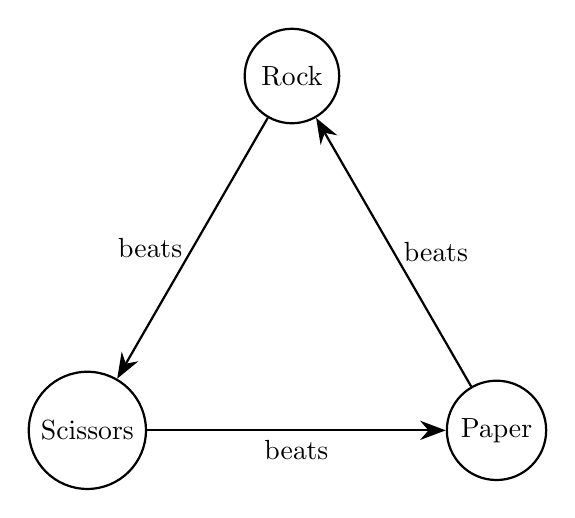
\begin{tikzpicture}[
    thick,
    ->,
    arrow style/.style={-{Stealth[scale=1.4]}},
    object/.style={circle, draw=black, thick, minimum size=1.2cm}
  ]

  % Nodes
  \node[object] (rock) at (90:3cm) {Rock};
  \node[object] (scissors) at (210:3cm) {Scissors};
  \node[object] (paper) at (330:3cm) {Paper};

  % Edges (no labels)
  \draw[arrow style] (rock) -- node [midway, left] {beats} (scissors);
  \draw[arrow style] (scissors) -- node [midway, below] {beats} (paper);
  \draw[arrow style] (paper) -- node [midway, right] {beats} (rock);

\end{tikzpicture}

}

\end{document}